\begin{frame}{Innovative Proposal: Nature's Solution}
    \begin{columns}
        % Colonna Testo (Sinistra)
        \begin{column}{0.52\textwidth}
            
            \begin{block}{The Feline Model}
                \textit{The Paw Pad} is a masterpiece of non-linear biomechanics, capable of adapting to varying impact velocities.
            \end{block}
            
            \vspace{0.2cm}
            
            \begin{block}{Anatomical Structure}
                \begin{enumerate}
                    \item \textbf{Epidermal:} Withstands intense ground interaction.
                    \item \textbf{Dermal:} Hydrostatic energy dissipation system.
                    \item \textbf{Subcutaneous:} Soft adipose tissue.
                \end{enumerate}

            \end{block}
            
            \vspace{0.2cm}
            
            \begin{alertblock}{Core Objective} % Riquadro di colore diverso (solitamente rosso/arancio)
                Translating this exact morphology into a prosthetic heel.
            \end{alertblock}
            
        \end{column}
        
        % Colonna Immagine (Destra)
        \begin{column}{0.45\textwidth}
            \hfill
            \begin{minipage}{0.9\textwidth}
                \centering
                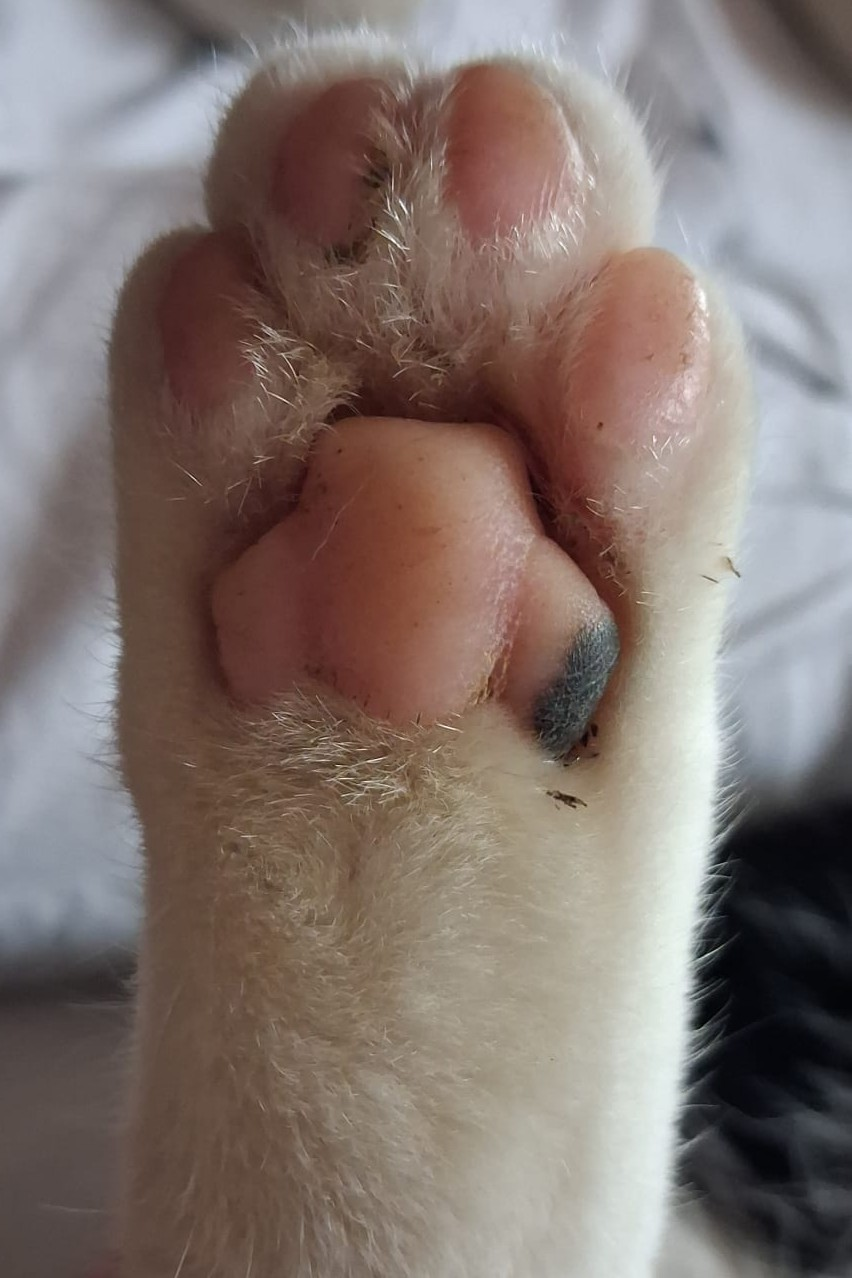
\includegraphics[width=\linewidth, height=0.45\textheight, keepaspectratio]{image/cat_pad.png}
                \vspace{0.4cm}
                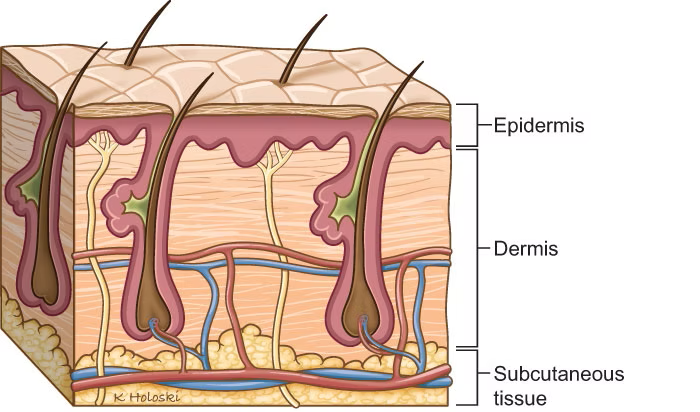
\includegraphics[width=\linewidth, height=0.35\textheight, keepaspectratio]{image/cat_layers.png}
            \end{minipage}
        \end{column}
    \end{columns}
\end{frame}